\chapter{\IfLanguageName{dutch}{Stand van zaken}{State of the art}}
\label{ch:stand-van-zaken}

Binnen de stand van zaken zal er verder ingegaan worden op de theoretische kant van deze bachelorproef. Hierbij zullen volgende thema's aanbod komen: Kotlin, de mogelijke ontwikkelingsvormen, Kotlin Multiplatform Mobile, de vergelijking met andere alternatieven en de gekozen testcriteria voor deze bachelorproef. De stand van zaken bouwt verder op de informatie uit de inleiding en versterkt deze aan de hand van de literatuurstudie. 

% Tip: Begin elk hoofdstuk met een paragraaf inleiding die beschrijft hoe
% dit hoofdstuk past binnen het geheel van de bachelorproef. Geef in het
% bijzonder aan wat de link is met het vorige en volgende hoofdstuk.

% Pas na deze inleidende paragraaf komt de eerste sectiehoofding.
%
%Dit hoofdstuk bevat je literatuurstudie. De inhoud gaat verder op de inleiding, maar zal het onderwerp van de bachelorproef *diepgaand* uitspitten. De bedoeling is dat de lezer na lezing van dit hoofdstuk helemaal op de hoogte is van de huidige stand van zaken (state-of-the-art) in het onderzoeksdomein. Iemand die niet vertrouwd is met het onderwerp, weet nu voldoende om de rest van het verhaal te kunnen volgen, zonder dat die er nog andere informatie moet over opzoeken \autocite{Pollefliet2011}.
%
%Je verwijst bij elke bewering die je doet, vakterm die je introduceert, enz. naar je bronnen. In \LaTeX{} kan dat met het commando \texttt{$\backslash${textcite\{\}}} of \texttt{$\backslash${autocite\{\}}}. Als argument van het commando geef je de ``sleutel'' van een ``record'' in een bibliografische databank in het Bib\LaTeX{}-formaat (een tekstbestand). Als je expliciet naar de auteur verwijst in de zin, gebruik je \texttt{$\backslash${}textcite\{\}}.
%Soms wil je de auteur niet expliciet vernoemen, dan gebruik je \texttt{$\backslash${}autocite\{\}}. In de volgende paragraaf een voorbeeld van elk.
%
%\textcite{Knuth1998} schreef een van de standaardwerken over sorteer- en zoekalgoritmen. Experten zijn het erover eens dat cloud computing een interessante opportuniteit vormen, zowel voor gebruikers als voor dienstverleners op vlak van informatietechnologie~\autocite{Creeger2009}.
%
%\lipsum[7-20]

\section{\IfLanguageName{dutch}{Kotlin}{Kotlin}}
\label{sec:SVZkotlin}



In juli 2011 kwam JetBrains, de maker van onder andere IntelliJ IDEA, naar buiten met een nieuw project genaamd Kotlin.\autocite{Jemerov2011} Kotlin is een algemene, cross-platform en statische taal met type-inferentie. \autocite{Oliveira2020} Hierbij verwijst de term algemene naar het feit dat Kotlin is ontwikkeld is voor allerlei verschillende types van software en in verschillende situaties kan gebruikt worden. Cross-platform gaat over het gegeven dat software kan bestaan in verschillende versies op meer dan één platform. Ook is er vernoemd dat Kotlin statische typering gebruikt als taal, dit komt neer op het feit dat Kotlin de types van de objecten zal controleren tijdens het compileren van de code en niet tijdens het uitvoeren. Andere talen die dezelfde strategie volgen zijn Java en C. Alsook zal Kotlin gebruik maken van type-inferentie, hiermee zal de taal zelf onderscheid kunnen maken tussen datatypes van bepaalde expressies. 

\section{\IfLanguageName{dutch}{Ontwikkelingsvormen}{Forms of development}}
\label{sec:SVZontwikkelingsvormen}


Allereerst moet de omschrijving van een platform besproken worden, een platform zal meestal een bepaalde programmeertaal, besturingssysteem of bepaalde hardware beschrijven. Dit kan ook een combinatie van meerdere zijn.\autocite{Bishop2006} Hiervan zijn enkele voorbeelden Java SE 15, hierbij wordt de taal bedoeld als platform. Een voorbeeld van een platform als besturingssysteem is bijvoorbeeld Windows 10 of MacOS Big Sur. Een voorbeeld hardware als platform is bijvoorbeeld een Intel of AMD processor. Uiteindelijk kan er ook gezegd worden dat een computer met als besturingssysteem Windows 10 en een laatste generatie Intel processor ook een specifiek platform is.
\\ \\
Eens de term platform duidelijker is, kan er makkelijker omschreven worden wat precies een cross-platform applicatie is en wat een native applicatie is. Een cross-platform applicatie is zoals de naam het al zegt een applicatie die op meerdere platformen zal werken. De software zal dus licht verschillende versies hebben die op hun beurt op allerlei verschillende platformen zullen werken. Native applicaties daarentegen zullen zich toespitsen op één bepaald platform.
\\ \\
Verder wordt er SWOT-analyse bekeken voor cross-platform applicaties. Deze sterkte-zwakteanalyse zal bekijken wat de sterktes en zwaktes zijn maar ook een beeld schetsen van de kansen en bedreigingen. Hiermee kunnen we een beeld schetsen wat de huidige positie is van cross-platform applicaties binnen de huidige markt. Uit onderzoek van Tommi Nivanaho naar cross-platform applicaties met React Native zijn een aantal factoren naar voor gekomen.\autocite{Nivanaho2019} Hier moet wel rekening gehouden worden met het feit dat sommige factoren niet toepasbaar zijn op alle cross-platform SDK’s en toolkits. Hieronder een overzicht van enkele punten uit de studie toepasbaar zijn op cross-platform applicaties in het algemeen.
\\
\begin{itemize}
    \item Sterktes of Strengths
    \begin{itemize}
        \item Sneller te ontwikkelen
        \item Kostenbesparend
        \item De applicatie ondersteunt meerdere platformen tegelijkertijd
    \end{itemize}
    \item Zwaktes of Weaknesses
    \begin{itemize}
        \item Nog steeds nood aan native code per platform
        \item Upgrades kunnen omslachtiger zijn
    \end{itemize}
    \item Kansen of Opportunities
    \begin{itemize}
        \item Snelle ontwikkeling voor meerdere platformen tegelijkertijd
        \item Native applicaties kunnen relatief vlot omgevormd worden naar cross-platform applicaties
    \end{itemize}
    \item Bedreigingen of Threats
    \begin{itemize}
        \item Updates aan het gekozen cross-platform systeem kunnen de reeds geschreven applicaties onbruikbaar maken
    \end{itemize}
\end{itemize}


\subsection{\IfLanguageName{dutch}{Native ontwikkeling}{Native development}}
\label{sec:SVZnative}

\subsection{\IfLanguageName{dutch}{Cross-platform ontwikkeling}{Cross-platform development}}
\label{sec:SVZcrossplatform}

\section{\IfLanguageName{dutch}{Multiplatform}{Multiplatform}}
\label{sec:SVZmultiplatform}


Kotlin Multiplatform is de nieuwe cross platform software development kit (SDK) van JetBrains. Ook werd een SDK uitgebracht specifiek gericht op de mobiele toestellen namelijk Kotlin Multiplatform Mobile (KMM). Kotlin Multiplatform werd voor het eerst verwerkt in Kotlin 1.2 in november 2017 als experimentele functie.\autocite{Jemerov2017} 
Ondertussen heeft de ontwikkeling van KMM niet stil gestaan en is in augustus 2020 de alpha versie van deze SDK uitgebracht voor het grote publiek.\autocite{Petrova2020} In november 2020 werd de 0.2.0 versie uitgebracht, deze is verwerkt in Kotlin 1.4.20.\autocite{JetBrains2020} Enkele delen van deze SDK en bijhorende componenten zijn nog steeds in de experimentele fase van ontwikkeling, maar JetBrains geeft aan dat het nu al een ideaal moment is om deze software te testen.\autocite{Petrova2020} De community achter KMM en het open source verhaal spelen hier een grote rol en zullen ook zorgen voor een snellere ontwikkeling van deze software. Bedrijven kunnen dus momenteel al experimenteel aan de slag met deze nieuwe software en voorbeelden van enkele bedrijven die de stap al hebben gezet naar KMM zijn onder andere Netflix, VMware en Autodesk.\autocite{KotlinKMMCaseStudies}

\subsection{\IfLanguageName{dutch}{Kotlin Multiplatform}{Kotlin Multiplatform}}
\label{sec:SVZKM}

\subsection{\IfLanguageName{dutch}{Kotlin Multiplatform Mobile}{Kotlin Multiplatform Mobile}}
\label{sec:SVZKMM}

\section{\IfLanguageName{dutch}{Kotlin Multiplatform versus alternatieven}{Kotlin Multiplatform versus alternatives}}
\label{sec:SVZKMMvsandere}
Kotlin Multiplatform (KM) zal het concept van cross-platform anders aanpakken dan andere alternatieven op de markt vandaag. Hierbij zit het verschil vooral in welke code van de applicatie zal gedeeld worden tussen de verschillende platformen. In de Kotlin documentatie staat beschreven hoe bepaalde delen van de code correct kunnen gedeeld worden tussen verschillende platformen. KM zal anders dan alternatieven de business logica delen tussen de verschillende platformen.\autocite{Kotlin2021} Hierbij wordt ook vermeld dat men enkel de business logica moet delen die gebruikt kan worden op alle platformen. 

\begin{figure}
    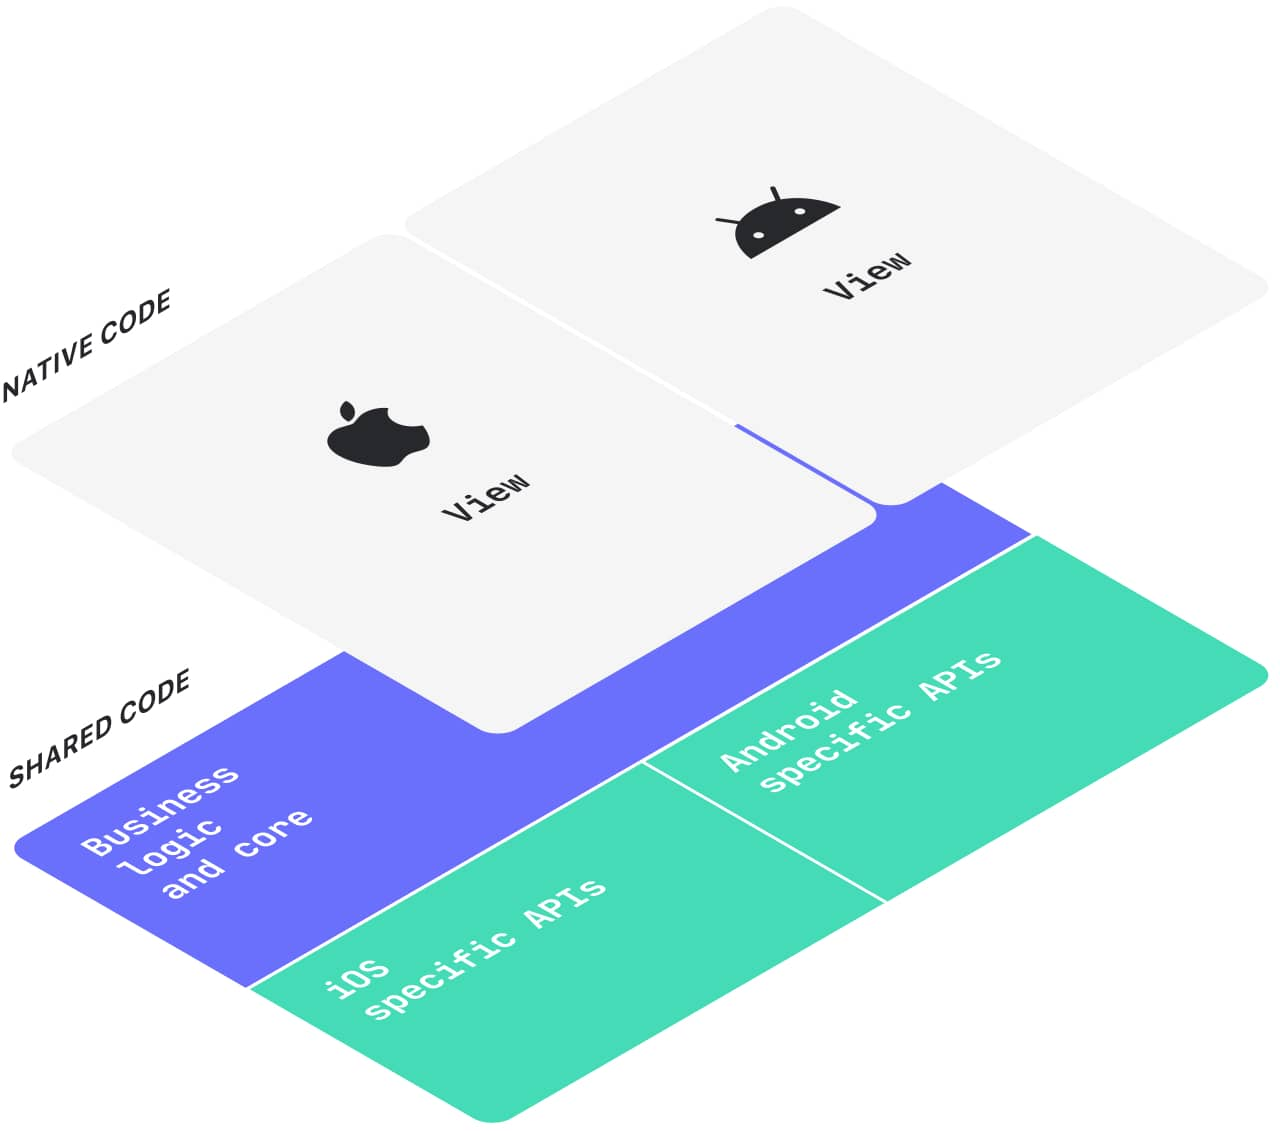
\includegraphics[width=\linewidth]{kmm.jpg}
    \caption{Grafische voorstelling Kotlin Multiplatform Mobile \autocite{KotlinKMM}}
    \label{fig:kmm}
\end{figure}

Figuur \ref{fig:kmm} geeft een goed algemeen beeld van de structuur van Kotlin Multiplatform Mobile. De ‘shared code’ in de figuur \ref{fig:kmm} verwijst hier naar Common Kotlin of CommonMain, dit is het gedeelde binnenin KM dat de gedeelde logica zal bevatten. Daarnaast zal er nog per platform een aparte main zijn die de code zal implementeren. Hier in de figuur \ref{fig:kmm} zal het project ook nog een iosMain en een kotlinMain, deze kunnen later ook nog uitgebreid worden met bijvoorbeeld een macosX64Main. De specifieke situatie in figuur \ref{fig:kmm} is een applicatie waar Kotlin Multiplatform Mobile gebruikt wordt. Deze zal zich speciaal richten op applicaties voor iOS en Android.
Voor de communicatie tussen het common deel en de platform specifieke delen zal Kotlin gebruik maken van het expected/actual systeem. Hierbij worden binnenin de CommonMain elementen gedeclareerd met expect en de platform specifieke delen zullen dezelfde elementen declareren met actual. Deze structuur kan gebruikt worden voor functies, klassen, interfaces, enumeraties, properties en annotaties. 
\\ \\
Nu er een beter beeld is geschetst van hoe KM, werkt zal er gekeken worden naar een mogelijk alternatief met een andere aanpak voor de gedeelde code, bijvoorbeeld Flutter. Flutter is een user interface toolkit ontwikkeld door Google en zit momenteel aan versie 1.22 sinds oktober 2020.\autocite{Sells2020} De toolkit richt zich op mobile, web en desktop applicaties en zal de code native compileren. Zoals reeds beschreven is Flutter een user interface toolkit en zal dus de user interface delen over de verschillende platformen. Hiervoor zal Flutter widgets gebruiken die geïnspireerd zijn door React.\autocite{FlutterWidgets} Dit impliceert dus dat hierbij de business logica zal moeten verwerkt worden per platform.
\\ \\
De developer kan dus kiezen om de user interface te delen onder de platformen en een toolkit te gebruiken zoals Flutter. Anderzijds kan er gekozen worden voor het delen van de business logica onder de platformen en dan kan KM gebruikt worden. Het delen van de user interface zal als voordeel hebben dat alle applicaties op de verschillende platformen dezelfde look en feel zullen hebben, echter is een nadeel dat de business logica per platform verwerkt zal moeten worden. Aan de kant van de gedeelde business logica is er het voordeel dat deze gedeeld is dus dat alle applicaties dezelfde logica hebben en implementeren, alsook kan er voor de user interface gebruik gemaakt worden van de platform specifieke frameworks. Er is echter ook een nadeel, hierbij kan gedacht worden aan het feit dat de user interface niet overal exact dezelfde zal zijn. 


\section{Testcriteria}
\label{sec:SVZtestcriteria}
Tijdens deze bachelorproef zullen van verschillende applicaties testcriteria geëvalueerd worden. Deze zullen ons vertellen in welke mate de cross-platform applicaties beter zijn dan de native. Volgende testcriteria werden gekozen voor deze vergelijkende studie.
\begin{itemize}
    \item Aantal lijnen code
    \begin{itemize}
        \item Het totaal aantal lijnen code van een applicatie zal geëvalueerd worden over het gehele project. In het geval van native applicaties zullen deze opgeteld worden met elkaar.
    \end{itemize}
    \item Kostprijs
    \begin{itemize}
        \item Hierbij wordt de geschatte kostprijs om een applicatie te laten ontwikkelen door een IT-bedrijf in kaart gebracht. Dit wordt berekend aan de hand van geschatte werkuren en een gemiddelde kostprijs per uur. Daarnaast wordt nagegaan of cross-platform een effect zal hebben op het systeem van vooraf bepaalde totaalprijzen indien bedrijven daarmee werken.
    \end{itemize}
    \item Ontwikkeltijd
    \begin{itemize}
        \item Deze tijd beschrijft het aantal werkuren dat een ontwikkelaar nodig heeft om een specifieke applicatie te schrijven. Hierbij kan onder andere gebruik gemaakt worden van platformen zoals GitHub om deze tijd te gaan meten of inschatten.
    \end{itemize}
    \item Compileersnelheid
    \begin{itemize}
        \item Dit is de snelheid waarmee de specifieke applicatie zal kunnen compileren en opstarten. Dit kan gemeten worden in de ontwikkelingssoftware voor de desbetreffende taal van de applicatie.
    \end{itemize}
    \item Voetafdruk
    \begin{itemize}
        \item Dit impliceert de omvang die de applicatie zal innemen op het platform waarvoor deze ontwikkeld is. Hiervoor kan de applicatie gebruikt worden die de ontwikkelingssoftware aanmaakt.
    \end{itemize}
    \item Uitbreiding van de applicatie
    \begin{itemize}
        \item Dit criterium kan geëvalueerd worden door vooraf bepaalde features van de applicatie weg te laten. Eens de applicatie klaar is voor productie kunnen deze features terug toegevoegd worden. Om de uitbreidbaarheid van de applicatie te gaan staven kan gebruik gemaakt worden van voorgaande testcriteria.
    \end{itemize}
\end{itemize}
